% Options for packages loaded elsewhere
\PassOptionsToPackage{unicode}{hyperref}
\PassOptionsToPackage{hyphens}{url}
%
\documentclass[
]{book}
\usepackage{amsmath,amssymb}
\usepackage{iftex}
\ifPDFTeX
  \usepackage[T1]{fontenc}
  \usepackage[utf8]{inputenc}
  \usepackage{textcomp} % provide euro and other symbols
\else % if luatex or xetex
  \usepackage{unicode-math} % this also loads fontspec
  \defaultfontfeatures{Scale=MatchLowercase}
  \defaultfontfeatures[\rmfamily]{Ligatures=TeX,Scale=1}
\fi
\usepackage{lmodern}
\ifPDFTeX\else
  % xetex/luatex font selection
\fi
% Use upquote if available, for straight quotes in verbatim environments
\IfFileExists{upquote.sty}{\usepackage{upquote}}{}
\IfFileExists{microtype.sty}{% use microtype if available
  \usepackage[]{microtype}
  \UseMicrotypeSet[protrusion]{basicmath} % disable protrusion for tt fonts
}{}
\makeatletter
\@ifundefined{KOMAClassName}{% if non-KOMA class
  \IfFileExists{parskip.sty}{%
    \usepackage{parskip}
  }{% else
    \setlength{\parindent}{0pt}
    \setlength{\parskip}{6pt plus 2pt minus 1pt}}
}{% if KOMA class
  \KOMAoptions{parskip=half}}
\makeatother
\usepackage{xcolor}
\usepackage{color}
\usepackage{fancyvrb}
\newcommand{\VerbBar}{|}
\newcommand{\VERB}{\Verb[commandchars=\\\{\}]}
\DefineVerbatimEnvironment{Highlighting}{Verbatim}{commandchars=\\\{\}}
% Add ',fontsize=\small' for more characters per line
\usepackage{framed}
\definecolor{shadecolor}{RGB}{248,248,248}
\newenvironment{Shaded}{\begin{snugshade}}{\end{snugshade}}
\newcommand{\AlertTok}[1]{\textcolor[rgb]{0.94,0.16,0.16}{#1}}
\newcommand{\AnnotationTok}[1]{\textcolor[rgb]{0.56,0.35,0.01}{\textbf{\textit{#1}}}}
\newcommand{\AttributeTok}[1]{\textcolor[rgb]{0.13,0.29,0.53}{#1}}
\newcommand{\BaseNTok}[1]{\textcolor[rgb]{0.00,0.00,0.81}{#1}}
\newcommand{\BuiltInTok}[1]{#1}
\newcommand{\CharTok}[1]{\textcolor[rgb]{0.31,0.60,0.02}{#1}}
\newcommand{\CommentTok}[1]{\textcolor[rgb]{0.56,0.35,0.01}{\textit{#1}}}
\newcommand{\CommentVarTok}[1]{\textcolor[rgb]{0.56,0.35,0.01}{\textbf{\textit{#1}}}}
\newcommand{\ConstantTok}[1]{\textcolor[rgb]{0.56,0.35,0.01}{#1}}
\newcommand{\ControlFlowTok}[1]{\textcolor[rgb]{0.13,0.29,0.53}{\textbf{#1}}}
\newcommand{\DataTypeTok}[1]{\textcolor[rgb]{0.13,0.29,0.53}{#1}}
\newcommand{\DecValTok}[1]{\textcolor[rgb]{0.00,0.00,0.81}{#1}}
\newcommand{\DocumentationTok}[1]{\textcolor[rgb]{0.56,0.35,0.01}{\textbf{\textit{#1}}}}
\newcommand{\ErrorTok}[1]{\textcolor[rgb]{0.64,0.00,0.00}{\textbf{#1}}}
\newcommand{\ExtensionTok}[1]{#1}
\newcommand{\FloatTok}[1]{\textcolor[rgb]{0.00,0.00,0.81}{#1}}
\newcommand{\FunctionTok}[1]{\textcolor[rgb]{0.13,0.29,0.53}{\textbf{#1}}}
\newcommand{\ImportTok}[1]{#1}
\newcommand{\InformationTok}[1]{\textcolor[rgb]{0.56,0.35,0.01}{\textbf{\textit{#1}}}}
\newcommand{\KeywordTok}[1]{\textcolor[rgb]{0.13,0.29,0.53}{\textbf{#1}}}
\newcommand{\NormalTok}[1]{#1}
\newcommand{\OperatorTok}[1]{\textcolor[rgb]{0.81,0.36,0.00}{\textbf{#1}}}
\newcommand{\OtherTok}[1]{\textcolor[rgb]{0.56,0.35,0.01}{#1}}
\newcommand{\PreprocessorTok}[1]{\textcolor[rgb]{0.56,0.35,0.01}{\textit{#1}}}
\newcommand{\RegionMarkerTok}[1]{#1}
\newcommand{\SpecialCharTok}[1]{\textcolor[rgb]{0.81,0.36,0.00}{\textbf{#1}}}
\newcommand{\SpecialStringTok}[1]{\textcolor[rgb]{0.31,0.60,0.02}{#1}}
\newcommand{\StringTok}[1]{\textcolor[rgb]{0.31,0.60,0.02}{#1}}
\newcommand{\VariableTok}[1]{\textcolor[rgb]{0.00,0.00,0.00}{#1}}
\newcommand{\VerbatimStringTok}[1]{\textcolor[rgb]{0.31,0.60,0.02}{#1}}
\newcommand{\WarningTok}[1]{\textcolor[rgb]{0.56,0.35,0.01}{\textbf{\textit{#1}}}}
\usepackage{longtable,booktabs,array}
\usepackage{calc} % for calculating minipage widths
% Correct order of tables after \paragraph or \subparagraph
\usepackage{etoolbox}
\makeatletter
\patchcmd\longtable{\par}{\if@noskipsec\mbox{}\fi\par}{}{}
\makeatother
% Allow footnotes in longtable head/foot
\IfFileExists{footnotehyper.sty}{\usepackage{footnotehyper}}{\usepackage{footnote}}
\makesavenoteenv{longtable}
\usepackage{graphicx}
\makeatletter
\def\maxwidth{\ifdim\Gin@nat@width>\linewidth\linewidth\else\Gin@nat@width\fi}
\def\maxheight{\ifdim\Gin@nat@height>\textheight\textheight\else\Gin@nat@height\fi}
\makeatother
% Scale images if necessary, so that they will not overflow the page
% margins by default, and it is still possible to overwrite the defaults
% using explicit options in \includegraphics[width, height, ...]{}
\setkeys{Gin}{width=\maxwidth,height=\maxheight,keepaspectratio}
% Set default figure placement to htbp
\makeatletter
\def\fps@figure{htbp}
\makeatother
\setlength{\emergencystretch}{3em} % prevent overfull lines
\providecommand{\tightlist}{%
  \setlength{\itemsep}{0pt}\setlength{\parskip}{0pt}}
\setcounter{secnumdepth}{5}
\usepackage{booktabs}

\usepackage{color}
\usepackage{framed}
\setlength{\fboxsep}{.8em}

% These colours were manually entered, they shouldn't matter unless you want pdf output

\newenvironment{redbox}{
  \definecolor{shadecolor}{RGB}{243, 154, 157}
  \color{white}
  \begin{shaded}}
 {\end{shaded}}

\newenvironment{bluebox}{
  \definecolor{shadecolor}{RGB}{172, 210, 237}
  \color{white}
  \begin{shaded}}
 {\end{shaded}}

\newenvironment{greenbox}{
  \definecolor{shadecolor}{RGB}{141, 181, 128}
  \color{white}
  \begin{shaded}}
 {\end{shaded}}
\ifLuaTeX
  \usepackage{selnolig}  % disable illegal ligatures
\fi
\usepackage[]{natbib}
\bibliographystyle{plainnat}
\usepackage{bookmark}
\IfFileExists{xurl.sty}{\usepackage{xurl}}{} % add URL line breaks if available
\urlstyle{same}
\hypersetup{
  pdftitle={{[}Name of Workshop{]}{[}Year{]}},
  pdfauthor={Instructors: {[}list instructor names here{]}},
  hidelinks,
  pdfcreator={LaTeX via pandoc}}

\title{{[}Name of Workshop{]}{[}Year{]}}
\author{Instructors: {[}list instructor names here{]}}
\date{{[}Insert dates of the workshop{]}}

\begin{document}
\maketitle

{
\setcounter{tocdepth}{1}
\tableofcontents
}
\part{Introduction}\label{part-introduction}

\chapter{Welcome}\label{welcome}

Welcome to CBW's {[}workshop name, year{]} Workshop!

Put some introductory content here. (ex. links to bioinformatics.ca, general info)

\chapter{Course Schedule}\label{course-schedule}

Copy paste a table into \url{https://www.tablesgenerator.com/markdown_tables} (select convert to markdown) to create a table in markdown.

\section{Pre-workshop Materials}\label{pre-workshop-materials}

Click \href{insert\%20link\%20here}{here} for your prework!

\section{Computing Setup \& Downloads}\label{computing-setup-downloads}

Insert downloads (ex. datasets) or other tech instructions here (ex. AWS Instructions)

\section{Meet Your Faculty}\label{meet-your-faculty}

Here's your team!

\subsection{Instructor, TA, \ldots{}}\label{instructor-ta}

\begin{quote}
Job Title
Company/University/\ldots{}
Location

--- contact information
\end{quote}

{[}insert description of the person{]}

\subsection{Michelle Brazas, PhD}\label{michelle-brazas-phd}

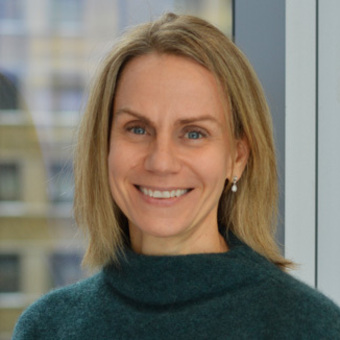
\includegraphics{./img/faculty/michelle-brazas.jpg}\\

\begin{quote}
Scientific Director
Canadian Bioinformatics Workshops (CBW)
Toronto, ON, CA

--- \href{mailto:support@bioinformatics.ca}{\nolinkurl{support@bioinformatics.ca}}
\end{quote}

Dr.~Michelle Brazas is the Associate Director for Adaptive Oncology at the Ontario Institute for
Cancer Research (OICR), and acting Scientific Director at Bioinformatics.ca. Previously, Dr.
Brazas was the Program Manager for Bioinformatics.ca and a faculty member in
Biotechnology at BCIT. Michelle co-founded and runs the Toronto Bioinformatics User Group
(TorBUG) now in its 11th season, and plays an active role in the International Society of
Computational Biology where she sits on the Board of Directors and Executive Board.

\subsection{Nia Hughes (she/her)}\label{nia-hughes-sheher}

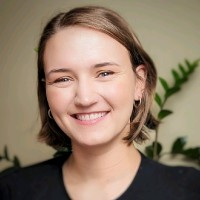
\includegraphics{./img/faculty/nia-hughes.jpeg}\\

\begin{quote}
Program Manager, Bioinformatics.ca
Ontario Institute for Cancer Research
Toronto, ON, Canada

--- \href{mailto:nia.hughes@oicr.on.ca}{\nolinkurl{nia.hughes@oicr.on.ca}}
\end{quote}

Nia is the Program Manager for Bioinformatics.ca, where she coordinates the Canadian
Bioinformatics Workshop Series. Prior to starting at OICR, she completed her M.Sc. in
Bioinformatics from the University of Guelph in 2020 before working there as a
bioinformatician studying epigenetic and transcriptomic patterns across maize varieties.

\section{Class Photo}\label{class-photo}

\textless- Replace the file address to your actual class photo file location

\part{Modules}\label{part-modules}

\chapter{Module 1}\label{module-1}

Welcome to module 1!

\section{Lecture}\label{lecture}

Here is an example of a pdf embedded:

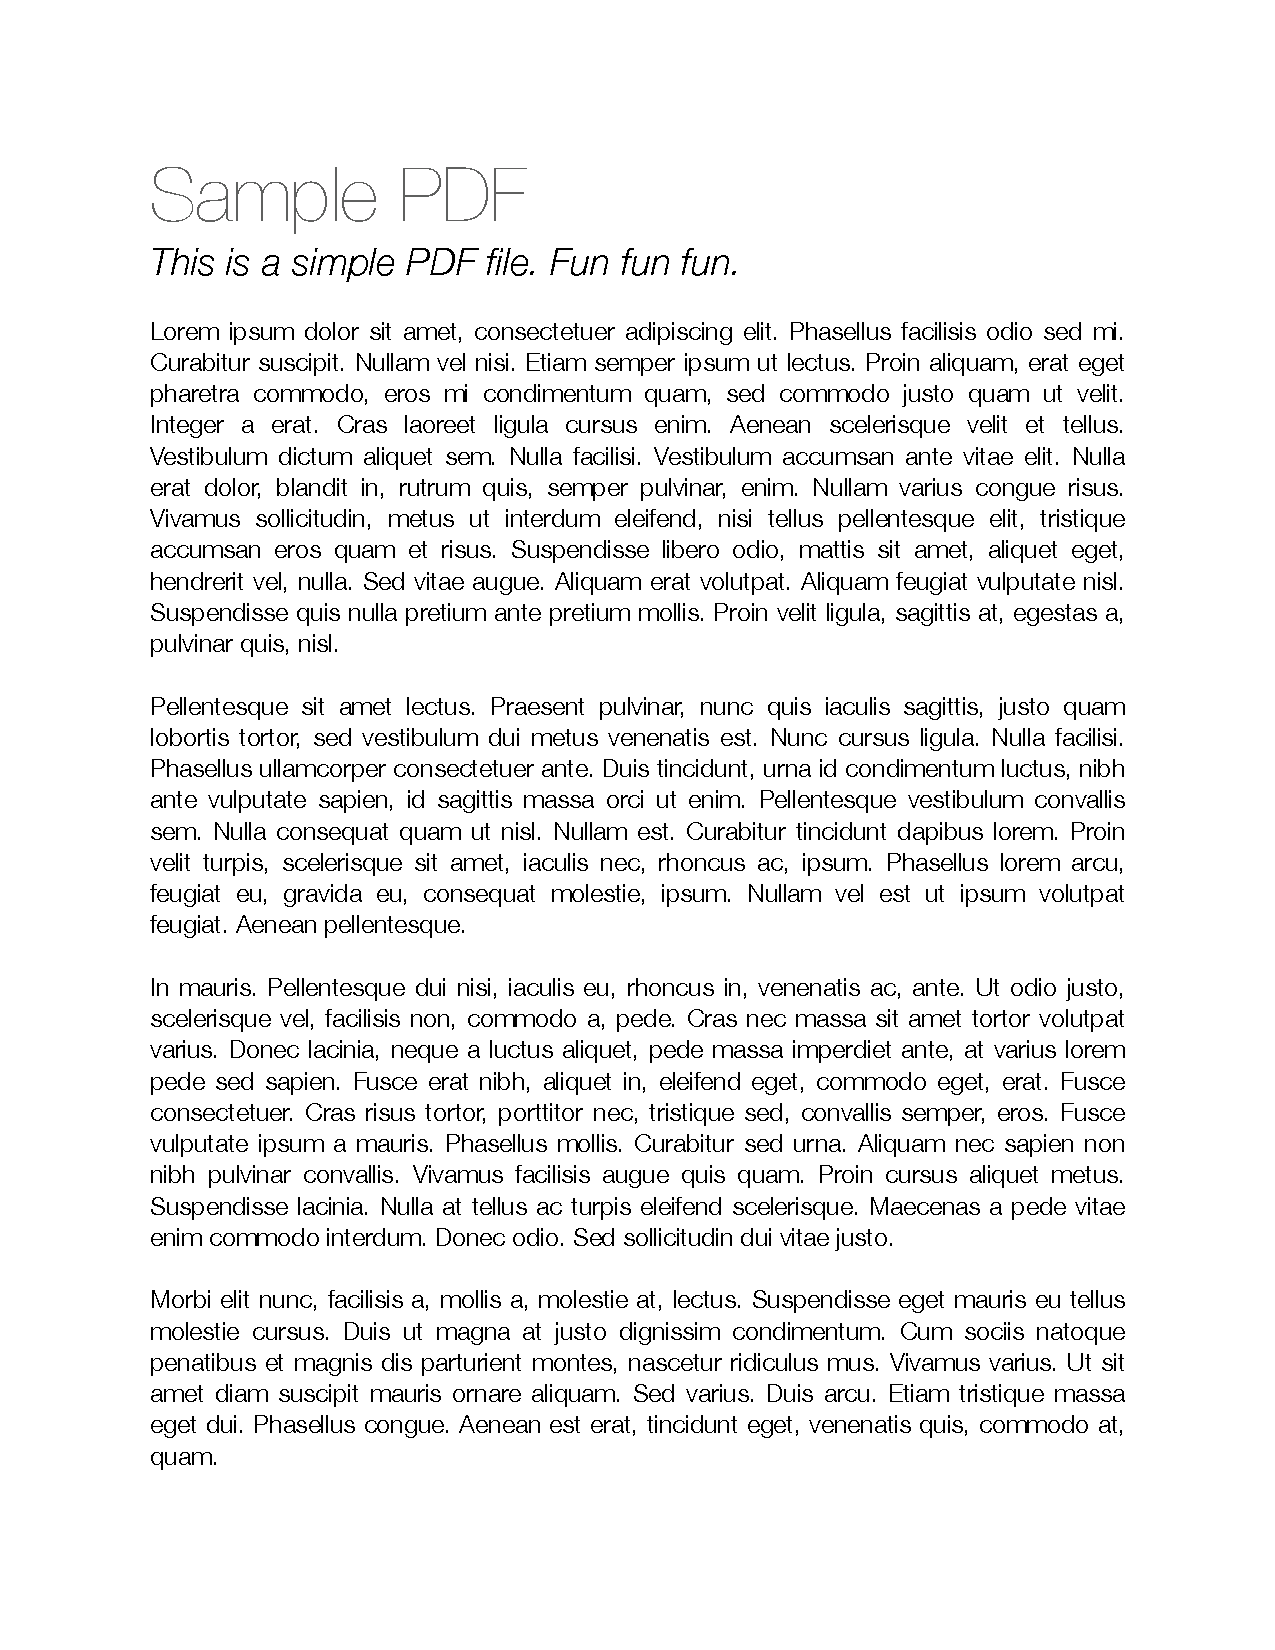
\includegraphics[width=1\textwidth,height=9.375in]{content-files/sample-pdf.pdf}~

Here is an example of a YouTube video embedded:

\^{} HEIGHT HAS A BUG

\subsection{Downloads}\label{downloads}

{[}insert your downloads for this module here (ex. datasets){]}

\section{Lab}\label{lab}

{[}Your lab here{]}

\begin{Shaded}
\begin{Highlighting}[]
\CommentTok{\# Your R code here}

\CommentTok{\# For example:}
\NormalTok{x }\OtherTok{\textless{}{-}} \DecValTok{42}
\NormalTok{x}
\end{Highlighting}
\end{Shaded}

\begin{verbatim}
## [1] 42
\end{verbatim}

\begin{Shaded}
\begin{Highlighting}[]
\CommentTok{\# Your python code here}

\CommentTok{\# For example:}
\BuiltInTok{print}\NormalTok{(}\StringTok{"hello world"}\NormalTok{)}
\end{Highlighting}
\end{Shaded}

\begin{verbatim}
## hello world
\end{verbatim}

\begin{Shaded}
\begin{Highlighting}[]
\CommentTok{\# Your bash code here}

\CommentTok{\# For example:}
\BuiltInTok{pwd}
\end{Highlighting}
\end{Shaded}

\begin{verbatim}
## /Users/jqiu/Documents/CBWgithub/cbw-dev-templates-docs/bookdown-template
\end{verbatim}

Try running these code ``chunks'' by pressing the green (left-pointing) triangle next to your code chunks.

You will see the code run in the console and the output provided below the code chunk.

The output of the code will also be produced under the code chunk on your website page.

\chapter{Module 2}\label{module-2}

\section{Lecture}\label{lecture-1}

\section{Lab}\label{lab-1}

\chapter{How to Render/Compile Code}\label{render-code}

There are many ways to render and compile code using Bookdown!

Here are most of the ``language engines'' (programming languages) available to render, run and compile in Bookdown!

\begin{Shaded}
\begin{Highlighting}[]
\FunctionTok{names}\NormalTok{(knitr}\SpecialCharTok{::}\NormalTok{knit\_engines}\SpecialCharTok{$}\FunctionTok{get}\NormalTok{())}
\end{Highlighting}
\end{Shaded}

\begin{verbatim}
##  [1] "awk"         "bash"        "coffee"      "gawk"        "groovy"     
##  [6] "haskell"     "lein"        "mysql"       "node"        "octave"     
## [11] "perl"        "php"         "psql"        "Rscript"     "ruby"       
## [16] "sas"         "scala"       "sed"         "sh"          "stata"      
## [21] "zsh"         "asis"        "asy"         "block"       "block2"     
## [26] "bslib"       "c"           "cat"         "cc"          "comment"    
## [31] "css"         "ditaa"       "dot"         "embed"       "eviews"     
## [36] "exec"        "fortran"     "fortran95"   "go"          "highlight"  
## [41] "js"          "julia"       "python"      "R"           "Rcpp"       
## [46] "sass"        "scss"        "sql"         "stan"        "targets"    
## [51] "tikz"        "verbatim"    "theorem"     "lemma"       "corollary"  
## [56] "proposition" "conjecture"  "definition"  "example"     "exercise"   
## [61] "hypothesis"  "proof"       "remark"      "solution"
\end{verbatim}

\section{Rendering Code}\label{rendering-code}

Just rendering code refers to Bookdown formatting code so that our users can view it. The code does not run or compile. This is very similar to what is shown in 020-module-1.Rmd of the bookdown template. An example is shown below.

\begin{verbatim}
```
insert code here
```
\end{verbatim}

which appears as

\begin{verbatim}
insert code here
\end{verbatim}

These are called ``code chunks''.

\section{Rendering Code with Highlights for Specific Languages}\label{rendering-code-with-highlights-for-specific-languages}

Bookdown also highlights (specific to the language) the outputted code for the ease of understanding. To do so, add the name of the language (of the many shown above) after the first 3 \texttt{\textasciigrave{}} symbols. Note that the language is not case sensitive (so both ``r'' and ``R'' would render the same below). For example:

\begin{verbatim}
```r
x <- 42
x
```
\end{verbatim}

renders into:

\begin{Shaded}
\begin{Highlighting}[]
\NormalTok{x }\OtherTok{\textless{}{-}} \DecValTok{42}
\NormalTok{x}
\end{Highlighting}
\end{Shaded}

Notice that since \texttt{\textless{}-} is how to assign values to variables in R, it is highlighted. If we were to replace ``r'' with a different language, this may not be highlighted (depending if ``\textless-'' is a relevant symbol in that language.)

\section{Rendering and Compiling Code}\label{rendering-and-compiling-code}

To have the code actually compile, we need to put ``\{'' and ``\}'' brackets around the language, which we still put after the first 3 \texttt{\textasciigrave{}} symbols. For example:

\begin{Shaded}
\begin{Highlighting}[]
\NormalTok{\textasciigrave{}\textasciigrave{}\textasciigrave{}\{r\}}
\NormalTok{x \textless{}{-} 42}
\NormalTok{x}
\NormalTok{htmltools::HTML(\textquotesingle{}\textless{}b\textgreater{}LEFT\textasciigrave{}RIGHT\textless{}/b\textgreater{}\textquotesingle{}) htmltools::HTML(\textquotesingle{}\textless{}b\textgreater{}LEFT\textasciigrave{}RIGHT\textless{}/b\textgreater{}\textquotesingle{}) htmltools::HTML(\textquotesingle{}\textless{}b\textgreater{}LEFT\textasciigrave{}RIGHT\textless{}/b\textgreater{}\textquotesingle{})}
\NormalTok{\textasciigrave{}\textasciigrave{}\textasciigrave{}}
\end{Highlighting}
\end{Shaded}

renders and compiles into:

\begin{Shaded}
\begin{Highlighting}[]
\NormalTok{x }\OtherTok{\textless{}{-}} \DecValTok{42}
\NormalTok{x}
\end{Highlighting}
\end{Shaded}

\begin{verbatim}
## [1] 42
\end{verbatim}

The second bar you see is the output of R command!

You can run these ``code chunks'' without previewing or building the book! To the right of your code chunk, there are 3 symbols (as seen below).

The {gear symbol} leads to more chunk options click on it to see more options.

The {down arrow symbol} runs all previous chunks and the current chunk. This is helpful if previous chunks define a variable that you will need in your current chunk.

\begin{quote}
\textbf{Note:} Hence, we can use variables from previous chunks!
\end{quote}

The {right-pointing arrow symbol} runs the current code chunk. A rectangular box will appear below your code chunk, with the output of your code.

Additionally, notice that in your bottom left window, any code you run also runs in your console. Both of these ways of checking your code happens for all languages! If you are previewing your book, you must re-preview it, since running the code becomes the new action for your console, instead of previewing the book.

\begin{redbox}

\begin{center}
\textbf{Note!}

\end{center}

If you want to run a certain language, you must have the language installed! R and python are already setup for you. (Python relies on the RStudio interface option, reticulate - you can reconfigure this if you'd like.) You may have to configure new languages so that they can run in RStudio, but generally, they should be able to run automatically.

\end{redbox}

\begin{bluebox}

\begin{center}
\textbf{Exiting the Console}

\end{center}

If you're running R, you don't have to exit the console (we already work in the R console when using Bookdown). However, if you're running a different language (for example, python), you will remain in the Python console, and must exit it to run Bookdown commands. You can look online for different ways to exit certain consoles, but generally running ``quit'' will return you to the R console.

\end{bluebox}

Now we know how to both render (just show) and compile (see the output) of our code!

\section{Code Chunk Options}\label{code-chunk-options}

Bookdown has options that we can include, to help with certain options for our code to appear and what it may produce.

Generally, the typical structure of adding code chunk options is shown below.

\begin{Shaded}
\begin{Highlighting}[]
\NormalTok{\textasciigrave{}\textasciigrave{}\textasciigrave{}\{r, option=VALUE, option=VALUE, ...\}}
\NormalTok{code}
\NormalTok{\textasciigrave{}\textasciigrave{}\textasciigrave{}}
\end{Highlighting}
\end{Shaded}

Some common code chunk options are:

\begin{itemize}
\tightlist
\item
  \texttt{echo}

  \begin{itemize}
  \tightlist
  \item
    \texttt{echo=TRUE} shows the code output (by default, it is on).
  \item
    \texttt{echo=FALSE} hides the code output.
  \end{itemize}
\item
  \texttt{eval}

  \begin{itemize}
  \tightlist
  \item
    \texttt{eval=TRUE} runs the code (default).
  \item
    \texttt{eval=FALSE} skips the chunk and does not execute the code.
  \end{itemize}
\item
  \texttt{results}

  \begin{itemize}
  \tightlist
  \item
    \texttt{results=\textquotesingle{}markup\textquotesingle{}} runs the code (default).
  \item
    \texttt{results=\textquotesingle{}asis\textquotesingle{}} leaves the output with no additional formatting.
  \item
    \texttt{results=\textquotesingle{}hide\textquotesingle{}} does not show the output.
  \end{itemize}
\item
  \texttt{include}

  \begin{itemize}
  \tightlist
  \item
    \texttt{include=TRUE} includes both the code and the output on your website (default).
  \item
    \texttt{include=FALSE} excludes both the code and the output on your website.
  \end{itemize}
\end{itemize}

Click here to find more code chunk options!

\section{Code Chunks for Code-Generated Figures and Tables}\label{code-chunks-for-code-generated-figures-and-tables}

We can use code chunks to help specify certain ways for code-generated figures and tables to appear, and how to link to them!

Generally, this will look like:

\begin{Shaded}
\begin{Highlighting}[]
\NormalTok{\textasciigrave{}\textasciigrave{}\textasciigrave{}\{r reference{-}name, option=VALUE, option=VALUE, ...\}}
\NormalTok{code that generates an image/table}
\NormalTok{\textasciigrave{}\textasciigrave{}\textasciigrave{}}
\end{Highlighting}
\end{Shaded}

Then, we can refer to the figure or table generated by the code in this chunk by using \texttt{\textbackslash{}@ref(fig:reference-name)} or \texttt{\textbackslash{}@ref(tab:chunk-label)}

For example, an R-generated image can be made using a similar code chunk to the one shown below:

\begin{Shaded}
\begin{Highlighting}[]
\NormalTok{See Figure \textbackslash{}@ref(fig:nice{-}fig).}

\NormalTok{\textasciigrave{}\textasciigrave{}\textasciigrave{}\{r nice{-}fig, fig.cap=\textquotesingle{}Here is a nice figure!\textquotesingle{}, out.width=\textquotesingle{}80\%\textquotesingle{}, fig.asp=.75, fig.align=\textquotesingle{}center\textquotesingle{}, fig.alt=\textquotesingle{}Plot with connected points showing that vapor pressure of mercury increases exponentially as temperature increases.\textquotesingle{}\}}
\NormalTok{par(mar = c(4, 4, .1, .1))}
\NormalTok{plot(pressure, type = \textquotesingle{}b\textquotesingle{}, pch = 19)}
\NormalTok{\textasciigrave{}\textasciigrave{}\textasciigrave{}}
\end{Highlighting}
\end{Shaded}

This renders into:

\begin{center}\rule{0.5\linewidth}{0.5pt}\end{center}

See Figure \ref{fig:nice-fig}.

\begin{Shaded}
\begin{Highlighting}[]
\FunctionTok{par}\NormalTok{(}\AttributeTok{mar =} \FunctionTok{c}\NormalTok{(}\DecValTok{4}\NormalTok{, }\DecValTok{4}\NormalTok{, .}\DecValTok{1}\NormalTok{, .}\DecValTok{1}\NormalTok{))}
\FunctionTok{plot}\NormalTok{(pressure, }\AttributeTok{type =} \StringTok{\textquotesingle{}b\textquotesingle{}}\NormalTok{, }\AttributeTok{pch =} \DecValTok{19}\NormalTok{)}
\end{Highlighting}
\end{Shaded}

\begin{figure}

{\centering 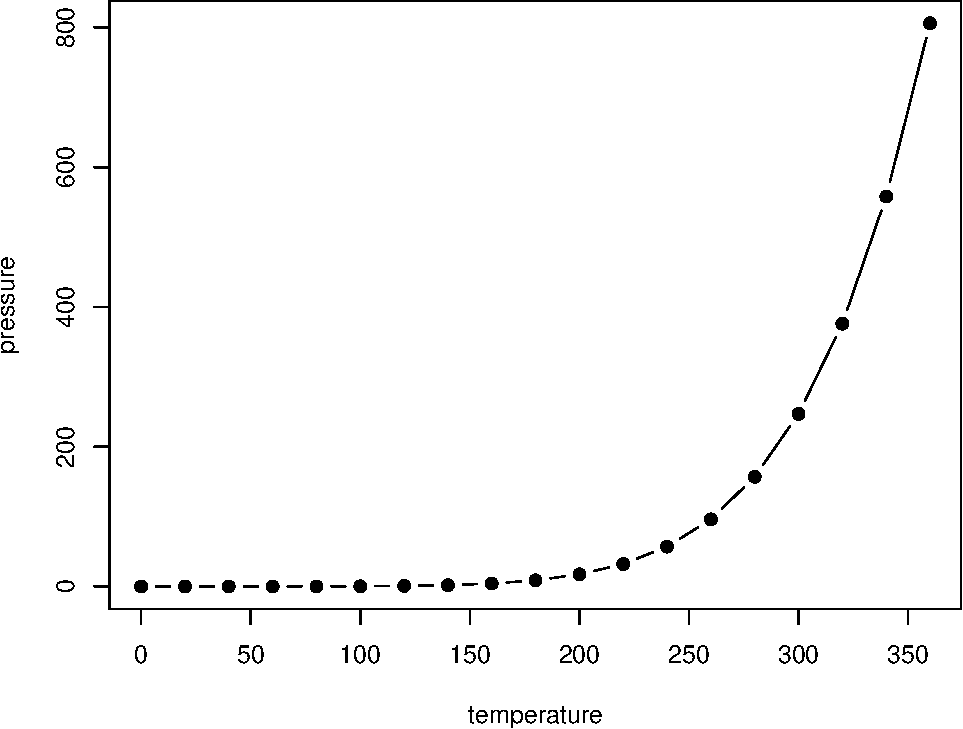
\includegraphics[width=0.8\linewidth,alt={Plot with connected points showing that vapor pressure of mercury increases exponentially as temperature increases.}]{_main_files/figure-latex/nice-fig-1} 

}

\caption{Here is a nice figure!}\label{fig:nice-fig}
\end{figure}

\begin{center}\rule{0.5\linewidth}{0.5pt}\end{center}

Here is an example of a table generated by R from a code chunk:

\begin{Shaded}
\begin{Highlighting}[]
\NormalTok{Don\textquotesingle{}t miss Table \textbackslash{}@ref(tab:nice{-}tab).}

\NormalTok{\textasciigrave{}\textasciigrave{}\textasciigrave{}\{r nice{-}tab, tidy=FALSE\}}
\NormalTok{knitr::kable(}
\NormalTok{  head(pressure, 10), caption = \textquotesingle{}Here is a nice table!\textquotesingle{},}
\NormalTok{  booktabs = TRUE}
\NormalTok{)}
\NormalTok{\textasciigrave{}\textasciigrave{}\textasciigrave{}}
\end{Highlighting}
\end{Shaded}

This renders into:

\begin{center}\rule{0.5\linewidth}{0.5pt}\end{center}

Don't miss Table \ref{tab:nice-tab}.

\begin{Shaded}
\begin{Highlighting}[]
\NormalTok{knitr}\SpecialCharTok{::}\FunctionTok{kable}\NormalTok{(}
  \FunctionTok{head}\NormalTok{(pressure, }\DecValTok{10}\NormalTok{), }\AttributeTok{caption =} \StringTok{\textquotesingle{}Here is a nice table!\textquotesingle{}}\NormalTok{,}
  \AttributeTok{booktabs =} \ConstantTok{TRUE}
\NormalTok{)}
\end{Highlighting}
\end{Shaded}

\begin{table}

\caption{\label{tab:nice-tab}Here is a nice table!}
\centering
\begin{tabular}[t]{rr}
\toprule
temperature & pressure\\
\midrule
0 & 0.0002\\
20 & 0.0012\\
40 & 0.0060\\
60 & 0.0300\\
80 & 0.0900\\
\addlinespace
100 & 0.2700\\
120 & 0.7500\\
140 & 1.8500\\
160 & 4.2000\\
180 & 8.8000\\
\bottomrule
\end{tabular}
\end{table}

\begin{center}\rule{0.5\linewidth}{0.5pt}\end{center}

You can find more inforamtion on figures and tables in Bookdown here!

  \bibliography{book.bib,packages.bib}

\end{document}
